\subsection{End-to-end case study using real ECG segments}
\label{sec:method-real-case}

The preceding small examples make the arithmetic manageable. This case study
now performs the operations on real archived ECG, using the research model
itself. It connects a normal-reference training window, an earlier labelled
PVC used for supervised fitting, and a later PVC withheld from fitting.
The waveforms are measured signals, and the reported predictions, residuals,
weights, and tree rules are calculated from the saved research artifacts.

Three kinds of evidence must be distinguished. The two-epoch autoencoder
losses and model-selection scores come from the original training logs.
The supervised forests were independently refitted on the complete original
development populations, reproducing every saved feature split, threshold,
and leaf value. A separate one-step autoencoder demonstration was run from
fresh random weights on real normal windows; this exposes an actual gradient
update but is not a reconstruction of an unrecorded historical training step.
The original saved models remain unchanged throughout.

\subsubsection*{1. Identify the signals and keep their roles separate}

The normal-reference example is the first four seconds of ECG1 from NSRDB
record 16272, one of the 15 fitting subjects. The supervised examples use
MLII from MITDB record 105. These are different databases, channels, and
training roles \cite{nsrdb,mitdb}. Table~\ref{tab:real-case-provenance} identifies
the segments so that the reader can locate them independently.

\begin{table}[H]
\centering
\small
\caption{Real ECG segments used in the training-to-prediction case study.}
\label{tab:real-case-provenance}
\begin{tabular}{@{}>{\raggedright\arraybackslash}p{3.5cm}
>{\raggedright\arraybackslash}p{3.5cm}
>{\raggedright\arraybackslash}p{5.7cm}@{}}
\toprule
Role & Source & Exact location and target\\
\midrule
Autoencoder demonstration & NSRDB 16272, ECG1 & Source samples 0--511 at
128 Hz; cached accepted window 0; clean waveform is the target.\\
\addlinespace
Supervised fitting example & MITDB 105, MLII & Accepted-beat index 484;
R peak 44,839 at 128 Hz (350.304688 s); binary target 1, subtype PVC.\\
\addlinespace
Temporal-test example & MITDB 105, MLII & Accepted-beat index 2,066;
R peak 187,009 at 128 Hz (1461.007813 s); annotation V, mapped to PVC.\\
\bottomrule
\end{tabular}
\end{table}

All indices in this case study are zero-based unless a residual-sum formula
explicitly uses the earlier one-based convention. Record 105 has 2,565
accepted beats, so its selection and test cuts are 1,641 and 2,052.
Candidate fitting uses indices 0--1,624; validation uses 1,641--2,035;
final refitting uses 0--2,035; and the test uses 2,052--2,564. The required
16-beat gaps precede validation during selection and the test during final
refitting. Thus index 484 can influence the learned rules, whereas index
2,066 cannot influence this rerun's fitting or model selection.

\begin{figure}[H]
\centering
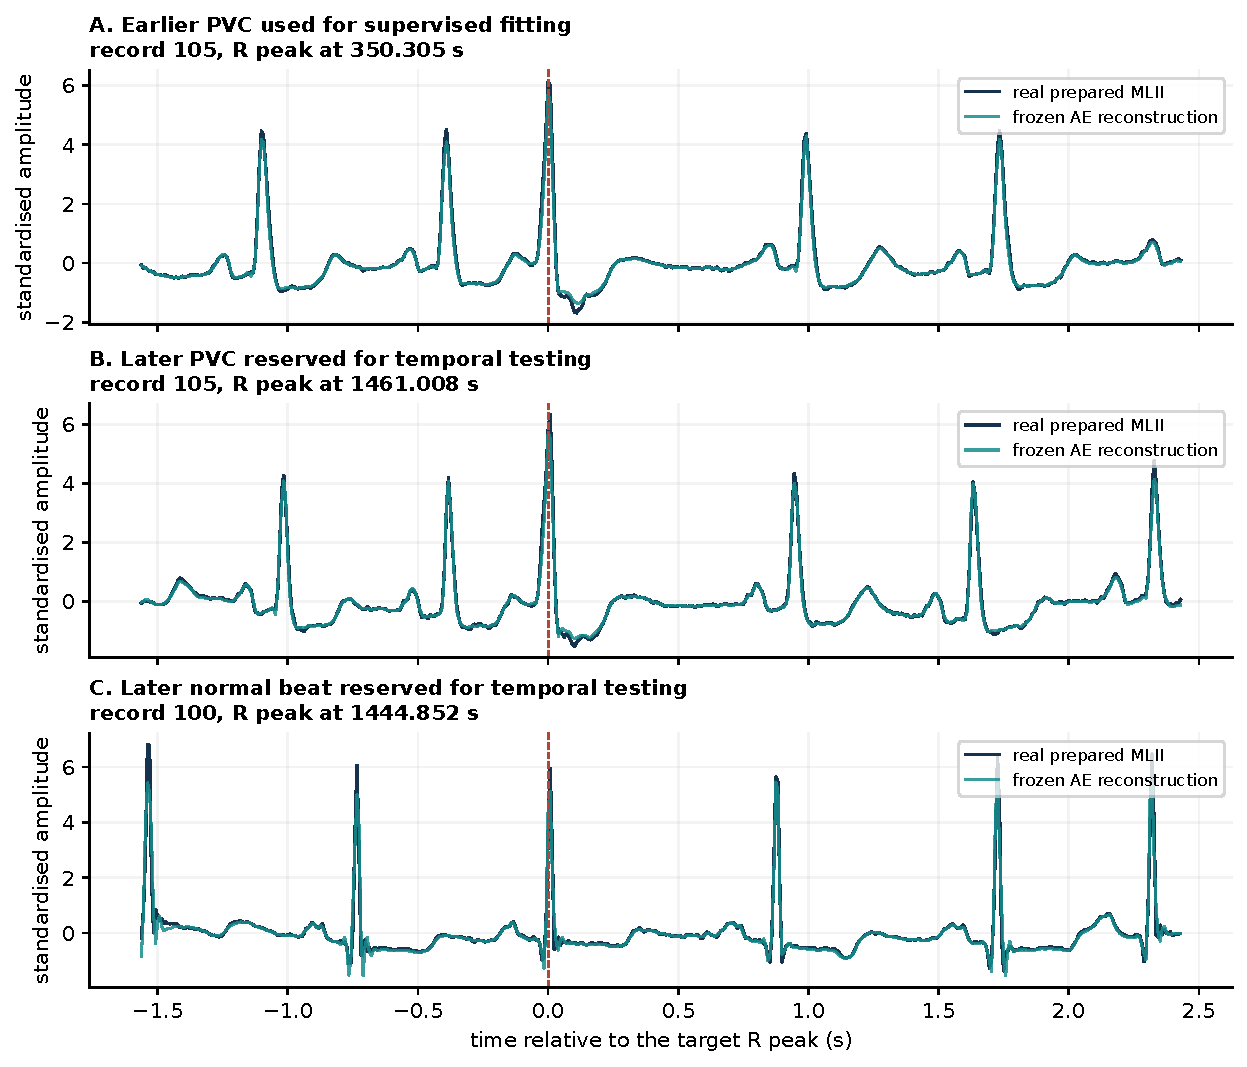
\includegraphics[width=.96\textwidth]{pic/generated/method_real_train_test_segments.pdf}
\caption[Real fitting and temporal-test ECG segments.]{Actual prepared ECG
windows and their saved-autoencoder reconstructions. The red line marks the
target R peak; the other peaks are neighbouring beats within the same
four-second window. Panels A and B are earlier and later PVC examples from
record 105. Panel C is a normal test beat from record 100. The classifier
labels the target beat, not every beat visible in the window.}
\label{fig:method-real-train-test}
\end{figure}

The examples were selected for explanation after the research models were
fixed. The test PVC is the first correctly classified PVC, in saved test
order, from a record that also contains candidate-fitting PVCs. The earlier
example is the middle candidate-fitting PVC in that record. This is a
transparent case-selection rule, not a new accuracy estimate. Patient overlap
and the earlier development exposure of the temporal test remain as described
in Chapter~\ref{ch:method}.

\subsubsection*{2. Observe a real autoencoder training update}

Training begins with normal data, before either classifier is fitted. The
first archived window from record 16272 is a real 512-value target. For
example, its first three clean samples are
$(-0.075544,-0.143846,-0.188566)$. In the new demonstration, Gaussian noise
with standard deviation 0.03 changes these inputs to
$(-0.103119,-0.150460,-0.140566)$. The clean values remain the targets.
Figure~\ref{fig:method-real-ae-training} shows the full segment rather than
only these three numbers.

\textbf{Preserve the archived scaling.} The saved first window has mean
0.005864 and standard deviation 0.530754. Consequently, its historical
scaling cannot be described as unit-variance scaling of that individual
window. Its waveform was matched to the filtered source samples using an
affine transformation, with maximum absolute discrepancy below
$1.1\times10^{-7}$. The demonstration uses the archived values directly;
silently standardising them again would change the training example. The
current normal-data preparation code specifies local standardisation when
rebuilding a cache, but it also reuses existing caches. That code alone does
not establish how an older cached array was scaled. This distinction does
not alter the verified beat-local scaling of the supervised MLII examples.

The demonstration uses the first 256 accepted cached windows from fitting
subject 16272, batch size 256, noise standard deviation 0.03, learning rate
0.001, and random seed 20260927. The network architecture is unchanged, but
its weights are freshly initialised. The noisy-input batch loss is
\begin{equation}
 \mathcal{L}_{\mathrm{before}}=
 \frac{1}{131072}\sum_{i=1}^{256}\sum_{t=1}^{512}
 (x_{it}-A_{\psi_0}(x_i+\epsilon_i)_t)^2
 =0.449509.
 \label{eq:real-ae-batch-loss}
\end{equation}
Here $131072=256(512)$ is the number of scalar reconstruction errors in
one batch. Every clean ECG sample contributes to the loss; no arrhythmia
label is supplied.

Backpropagation gives the actual gradient $-0.610003$ for the final output
bias. Its value before the update is $-0.147403$. At this first Adam step,
the moment calculations and bias correction give
\begin{align}
 m_1&=0.1(-0.610003)=-0.0610003,\\
 v_1&=0.001(-0.610003)^2\approx0.000372103,\\
 (\widehat m_1,\widehat v_1)&\approx(-0.610003,0.372103),\\
 b_{\mathrm{out},1}
 &=-0.147403-0.001\frac{-0.610003}{\sqrt{0.372103}+10^{-8}}
 \approx-0.146403.
 \label{eq:real-ae-bias-update}
\end{align}
This is one visible parameter change among all the network updates. Its
negative gradient moves the bias upward to reduce the batch error locally.
The filters and normalisation parameters receive their own gradients;
changing only this bias would not reproduce the complete training step.

Re-evaluating the same noisy batch with the same dropout masks after the
update gives MSE 0.319433. The displayed window's own MSE changes from
0.435649 to 0.313658. The controlled comparison shows that this particular
update reduced the error. It does not imply that one step learns normal ECG
adequately or that every future step reduces every window's error.

\begin{figure}[H]
\centering
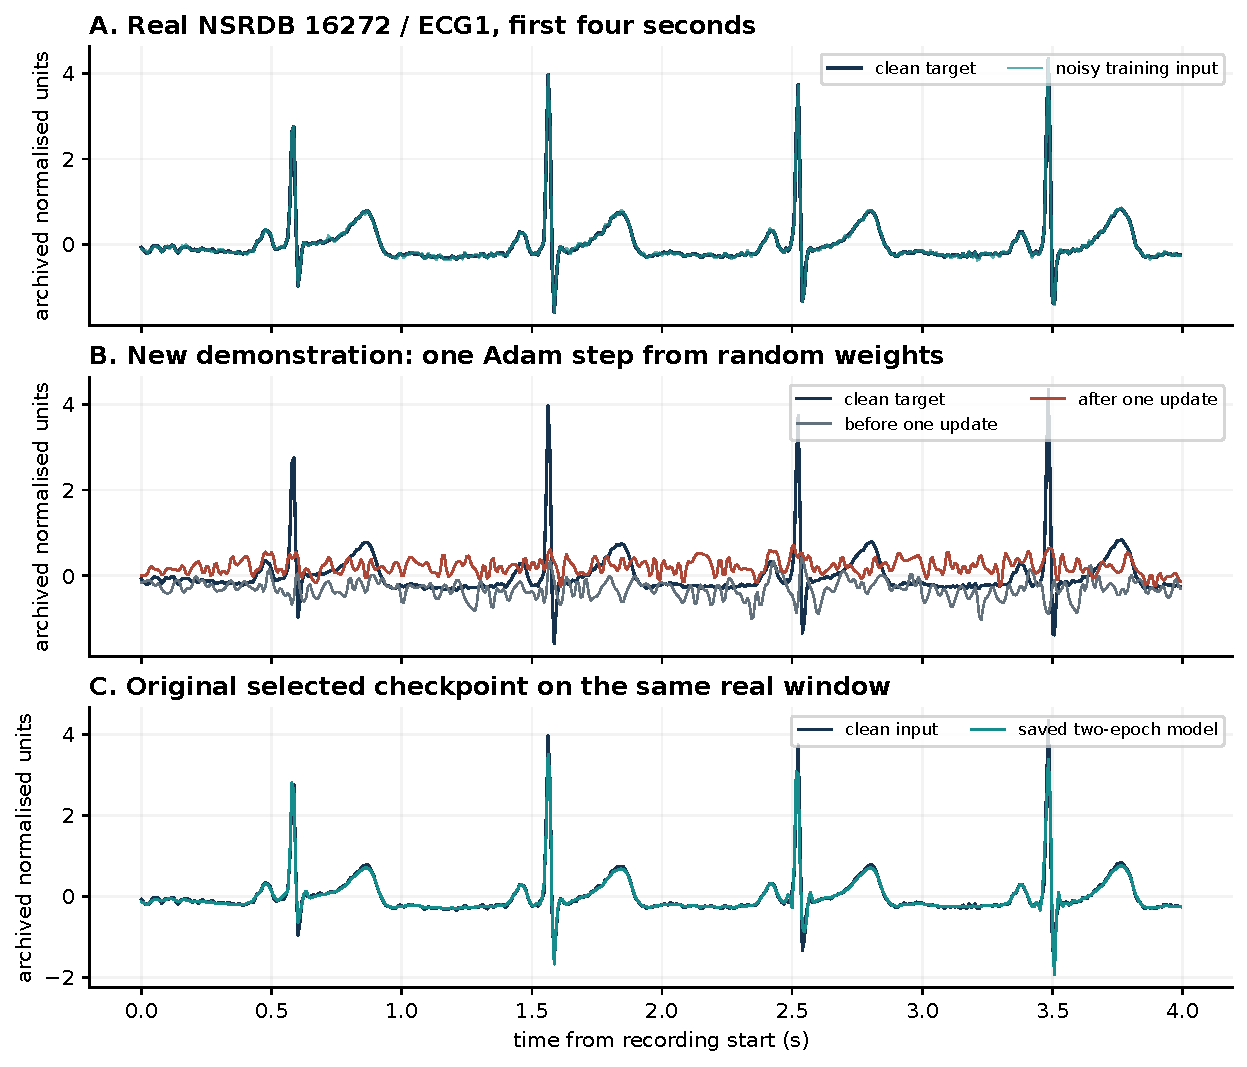
\includegraphics[width=.96\textwidth]{pic/generated/method_real_ae_training.pdf}
\caption[Real ECG through one training update and the saved autoencoder.]{Real
ECG1 samples from NSRDB 16272. A: clean target and newly corrupted input.
B: actual outputs before and after one isolated Adam update from random
weights. C: reconstruction by the original selected two-epoch checkpoint.
Panel C is not the result of the single step in panel B. Archived normalised
amplitudes are retained.}
\label{fig:method-real-ae-training}
\end{figure}

The original full training used 288,673 fitting windows, shuffled across
15 subjects, for two epochs. Each epoch therefore contained 1,128 batches,
including a smaller final batch. Its recorded training MSE was 0.057639 and
0.041976; clean-input validation MSE on the three other subjects was
0.061195 and 0.061193. The second checkpoint was retained. On the displayed
normal fitting window, that checkpoint has MSE 0.010463, as illustrated in
panel C. This last number describes a fitting example, not unseen-subject
performance. The independently measured validation loss remains the evidence
used to choose the checkpoint.

\subsubsection*{3. Convert real labelled beats into supervised feature rows}

Once the autoencoder is frozen, earlier MLII beats become the examples used
to train the two forests. The fitting PVC at 350.304688 seconds supplies
one 242-value row, binary target 1, and subtype target PVC. Its previous and
next RR intervals are 0.398438 and 0.992188 seconds, and its four residual
features are
\begin{equation}
 a_{\mathrm{fit}}=(0.052354,0.011190,0.065462,0.041013).
 \label{eq:real-training-residuals}
\end{equation}
These numbers are computed from the waveform in panel A of
Figure~\ref{fig:method-real-train-test}. Normal fitting beats supply the same
kind of feature row with binary target 0. Other supported abnormalities
supply binary target 1 and their own subtype target. The training populations
contain many such rows; the forests are not fitted to just the displayed PVC.

The later test PVC follows the identical feature calculation, but its label
is withheld from fitting. Its original annotation is V at source sample
525,964 in the 360 Hz recording. Resampling and index conversion give
\begin{equation}
 s_* = \left\lfloor525964\frac{128}{360}\right\rfloor=187009,
 \qquad u_*=v[186809:187321].
 \label{eq:real-window-extraction}
\end{equation}
The slice endpoint is exclusive: samples 186,809 through 187,320 provide
exactly 512 values. The R peak appears at local index 200. After filtering,
the window mean and standard deviation are 0.018076 and 0.325109 mV.
For example, the filtered sample at the target peak is 1.903376 mV, so
\begin{equation}
 x_*[200]=\frac{1.903376-0.018076}{0.325109+10^{-8}}
 \approx5.798973.
 \label{eq:real-peak-scaling}
\end{equation}
The values printed here are rounded; computations use full precision.
Standardisation changes the amplitude units, while preserving the relative
shape shown in Figure~\ref{fig:method-real-prediction}.

The first eight standardised samples have mean $-0.024118$, giving feature
entry 0. The mean of samples 216--223 is $-1.222917$, giving entry 27.
The 12--20 Hz log-relative-power measurement is 0.111020 at entry 208.
These are examples of actual waveform-derived values, rather than manually
assigned descriptions such as ``wide QRS''. The remaining waveform entries
are calculated by the same pooling, spectrum, and statistics rules.

The observed neighbouring peaks are 186,960 and 187,130. Their timing gives
\begin{align}
 \Delta_*&=(187009-186960)/128=0.3828125\ \mathrm{s},\\
 \Delta_{*+1}&=(187130-187009)/128=0.9453125\ \mathrm{s}.
 \label{eq:real-rr-intervals}
\end{align}
The short preceding interval and longer following interval describe the
timing around this annotated premature beat. They are measurements used by
the model, not a stand-alone diagnostic rule. The local mean of the preceding
ten intervals is 0.635156 seconds. Hence the previous/local-mean ratio is
$0.3828125/0.63515625=0.602706$, the next/local-mean ratio is 1.488315,
and instantaneous rate is $60/0.3828125=156.7347$ beats per minute.
This rate is the reciprocal of one interval, not a long-term average rate.

\begin{table}[H]
\centering
\small
\caption{All 15 measured RR features for the real temporal-test PVC.}
\label{tab:real-rr-values}
\begin{tabular}{@{}lrlr@{}}
\toprule
Base measurement & Value & History measurement & Value\\
\midrule
Previous RR (s) & 0.382813 & Median (s) & 0.656250\\
Next RR (s) & 0.945313 & IQR (s) & 0.039063\\
Local mean RR (s) & 0.635156 & MAD (s) & 0.019531\\
Previous / local mean & 0.602706 & RMSSD (s) & 0.062884\\
Next / local mean & 1.488315 & pNN50 fraction & 0.052632\\
RR coefficient of variation & 0.136199 & Range / median & 0.476190\\
Instantaneous rate (bpm) & 156.734695 & Normalised trend & $-0.004654$\\
 & & Normalised latest change & $-0.392857$\\
\bottomrule
\end{tabular}
\end{table}

The 20-interval history contains 19 successive differences. Exactly one
exceeds 0.05 seconds in absolute value, so pNN50 is $1/19=0.052632$.
This explains both the denominator and why the stored value is a fraction.
The full history and all 242 feature entries are retained in the case-study
audit file identified at the end of this subsection.

The frozen autoencoder reconstructs the same test window. Its measured
absolute-residual sum is 27.777321 and squared-residual sum is 6.070283.
Applying the residual equations gives
\begin{align}
 a_{*,1}&=27.777321/512=0.054253, &
 a_{*,2}&=6.070283/512=0.011856,\\
 a_{*,3}&=14.046151/240=0.058526, &
 a_{*,4}&=30.254937/511=0.059207.
 \label{eq:real-test-residuals}
\end{align}
These four numbers are appended after the 223 waveform and 15 RR values.
The archived feature row was independently rebuilt from the source signal,
measured peak context, and saved checkpoint. Recomputed residuals agreed
with the saved values within $2\times10^{-6}$, and the saved forests returned
the same scores from the rebuilt row.

\begin{figure}[H]
\centering
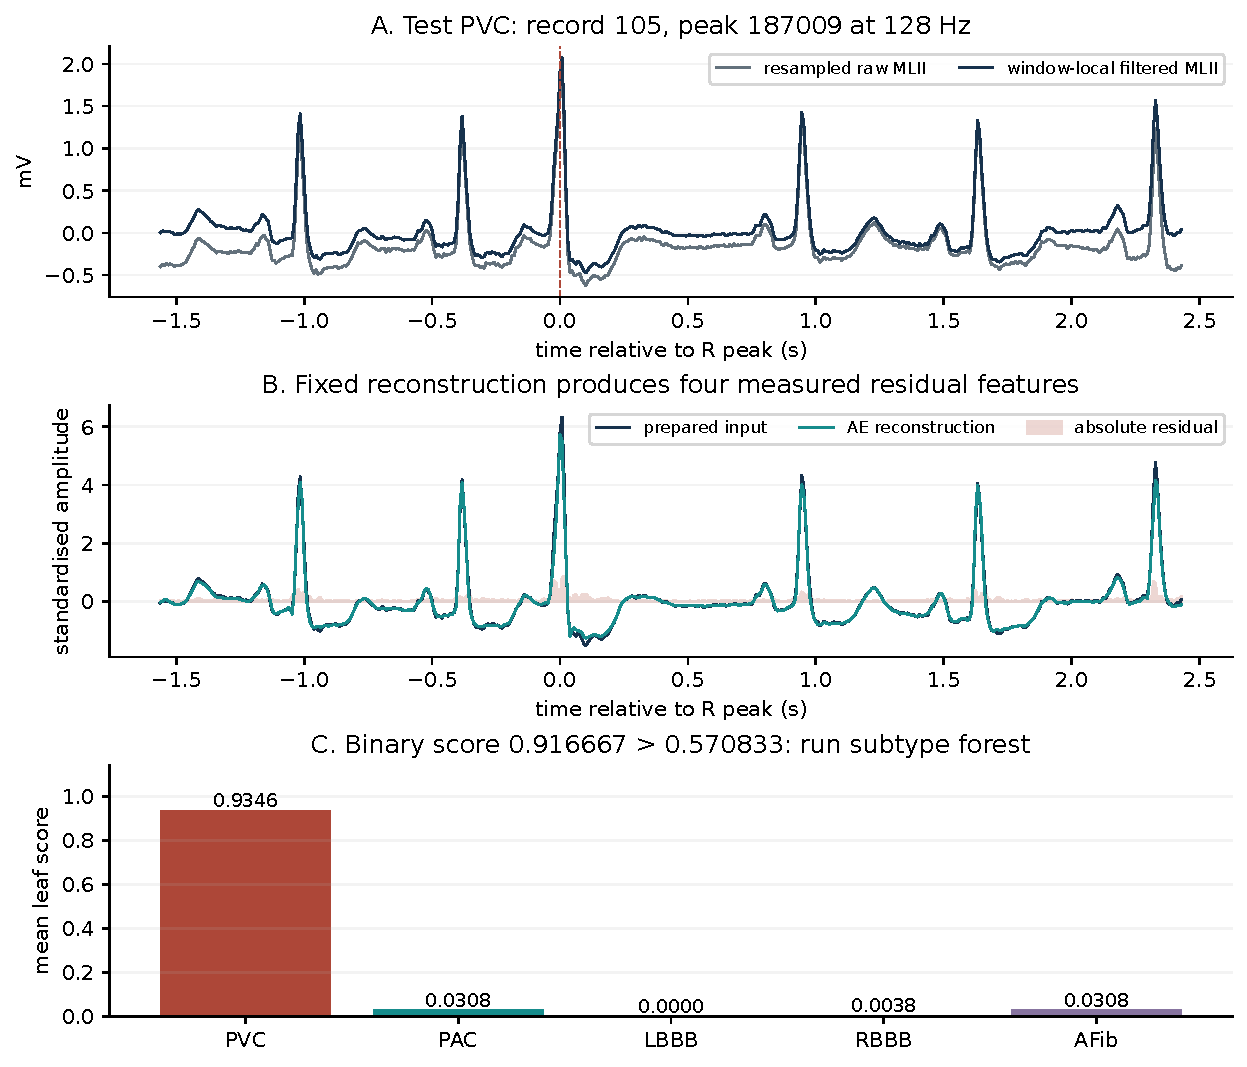
\includegraphics[width=.96\textwidth]{pic/generated/method_real_prediction_walkthrough.pdf}
\caption[Real test PVC from source ECG to subtype scores.]{The same real test
PVC passes through source-window filtering, standardisation, frozen
autoencoder reconstruction, and the two supervised forests. The bottom
panel reports measured subtype scores after the binary gate passes the beat.
The expert V annotation is used for comparison, not supplied to prediction.}
\label{fig:method-real-prediction}
\end{figure}

An important observation is that the autoencoder reconstructs this abnormal
beat quite closely. Its MAE is 0.054253, while the displayed normal test
beat has a larger MAE of 0.095564. Thus these real examples do not support
the shortcut ``larger reconstruction error always means abnormal''. The
forests use the joint morphology, rhythm, and residual evidence. The
autoencoder alone does not determine either the binary decision or the PVC
subtype.

\subsubsection*{4. Learn the binary forest from real development rows}

For final refitting, every eligible development row receives a binary target
and a sample weight. The displayed fitting PVC belongs to the abnormal
class, which contains 32,477 development beats across 42 subject clusters.
Record 105 contributes 39 abnormal development beats. Its unnormalised
binary weight is therefore
\begin{equation}
 \widetilde w_B=\frac{1}{32477}
 \left(\frac{32477}{42(39)}\right)^{0.35}
 \approx8.75923\times10^{-5}.
 \label{eq:real-binary-weight}
\end{equation}
Dividing by the mean weight across all 83,050 binary fitting rows and applying
the clipping rule gives $w_B=4.073719$. The displayed beat therefore has
more influence than a row with weight one. It is still one real beat; the
weight does not create copies or add new observations.

Consider the first tree in the final binary forest. At its root, the total
weight is 83,050 and the weighted class shares are
$(0.524047,0.475953)$ for N and abnormal. Their entropy is 0.998331 bits.
The fitted split asks whether whole-window mean bin 27 is at most
1.150551. The left child receives 82,227 rows with total weight 81,919.375851;
the right child receives 823 rows with weight 1,130.624149. Their entropies
are 0.997322 and 0.326286. Substituting actual fitted-node values gives
\begin{equation}
 \begin{aligned}
 \Delta H_B={}&0.998331
 -\frac{81919.375851}{83050}(0.997322)\\
 &-\frac{1130.624149}{83050}(0.326286)
 \approx0.010144\ \text{bits}.
 \end{aligned}
 \label{eq:real-binary-root-gain}
\end{equation}
This modest reduction is a real first partition, not the final classification.
The algorithm compares randomly proposed splits, retains the best available
one, and repeats the operation inside each child. Different features become
useful later in the tree. The saved tree records the winning rules; it does
not retain the full historical list of rejected candidate splits.

The 240-tree forest repeats this learning process with different random
choices. All trees receive the same weighted development population because
bootstrap sampling is disabled. No derivative of the autoencoder is computed
during tree fitting, and the two supervised targets never change the frozen
autoencoder checkpoint.

\subsubsection*{5. Learn the subtype forest from real abnormal rows}

Subtype fitting keeps only the 28,758 supported abnormal development beats.
The displayed fitting PVC now belongs to a class containing 5,632 PVC beats
across 32 subject clusters; record 105 contributes 35 PVC development beats.
The subtype weight calculation is
\begin{equation}
 \widetilde w_C=\frac{1}{5632}
 \left(\frac{5632}{32(35)}\right)^{0.25}
 \approx2.65888\times10^{-4},\qquad w_C=1.693698.
 \label{eq:real-subtype-weight}
\end{equation}
The different final weight arises because both the target classes and the
fitting population differ. The same feature row can therefore have weight
4.073719 in binary fitting and 1.693698 in subtype fitting.

At the root of the first subtype tree, the weighted shares for PVC, PAC,
LBBB, RBBB, and AFib are
$(0.193628,0.159765,0.221019,0.210692,0.214895)$.
The entropy is 2.312778 bits. This tree's first split uses RR pNN50, with
threshold 0.678082. The left and right children contain 16,935 and 11,823
rows, have weights 18,528.763857 and 10,229.236143, and have entropies
2.111793 and 1.685630. Thus
\begin{equation}
 \begin{aligned}
 \Delta H_C={}&2.312778
 -\frac{18528.763857}{28758}(2.111793)\\
 &-\frac{10229.236143}{28758}(1.685630)
 \approx0.352572\ \text{bits}.
 \end{aligned}
 \label{eq:real-subtype-root-gain}
\end{equation}
This calculation separates mixtures of abnormal subtypes. It never asks
whether a beat is N, because N is absent from this fitting population.
Further nodes combine frequency, morphology, and rhythm features until
leaves store their weighted subtype shares. Averaging 260 such trees gives
the final five-score vector.

\subsubsection*{6. Use validation to select models, then freeze the refits}

The foregoing final-tree calculations follow model selection. During the
original selection stage, the candidate forests learned from the earlier
candidate-fitting regions and were compared on the later validation regions.
Table~\ref{tab:real-candidate-selection} gives their recorded scores. These
are original experiment measurements, not the small illustrative scores
used earlier in this section.

\begin{table}[H]
\centering
\small
\caption{Recorded validation measurements selecting the real saved models.}
\label{tab:real-candidate-selection}
\begin{tabular}{@{}llrrr@{}}
\toprule
Stage & Candidate & Threshold & Primary score & Secondary score\\
\midrule
Binary & depth14 & 0.504692 & BA 0.976183 & F1 0.969381\\
Binary & depth22 & 0.536820 & BA 0.985738 & F1 0.981085\\
Binary & deep (selected) & 0.570833 & BA 0.987304 & F1 0.983886\\
\addlinespace
Subtype & depth22 & -- & Macro F1 0.978043 & Accuracy 0.986197\\
Subtype & deep\_sqrt & -- & Macro F1 0.976246 & Accuracy 0.985135\\
Subtype & deep\_third (selected) & -- & Macro F1 0.981126 & Accuracy 0.988321\\
\bottomrule
\end{tabular}
\end{table}

The deep binary candidate has the highest validation balanced accuracy, and
the deep\_third subtype candidate has the highest validation macro F1.
Their settings are retained. Final refitting then uses all eligible earlier
development rows, with fresh weights for those populations. The fixed
binary threshold remains $0.5708333333333333$; test labels do not choose it.

For this case study, the full 240-tree and 260-tree refits were reproduced
in memory using their original final-fitting seeds 20260901 and 20260902.
Every feature index, split threshold, and leaf-value array matched the saved
forests exactly. Predictions over all 20,969 temporal-test rows also matched
within numerical tolerance. This verifies the connection between the stated
training procedure and the particular models used below. It does not add an
independent test population or remove the original study's design limitations.

\subsubsection*{7. Route the later real PVC through the learned trees}

Now place the training labels aside. The later test beat contributes only
its prepared feature row $z_*$. A learned tree does not compare it with a
stored ECG picture; it applies its feature thresholds in order. In the first
binary tree, feature entry 27 is $-1.222917$, so it satisfies
$-1.222917\leq1.150551$ and takes the left branch. At the next node,
entry 28 is $-0.617664$, which is greater than $-1.485152$, so it takes
the right branch. Table~\ref{tab:real-binary-path} records every subsequent
comparison in this tree. Feature entry 27 means the 28th value in the
242-entry vector; feature and node indices here follow the zero-based code.

{\small
\begin{longtable}{@{}r>{\raggedright\arraybackslash}p{4.0cm}rrl@{}}
\caption{Complete route of the real test PVC through the first saved binary tree.}
\label{tab:real-binary-path}\\
\toprule
Node & Feature (zero-based index) & Beat value & Split value & Branch\\
\midrule
\endfirsthead
\toprule
Node & Feature (zero-based index) & Beat value & Split value & Branch\\
\midrule
\endhead
\bottomrule
\endfoot
0 & 27: whole-window mean bin 27 & $-1.222917$ & $1.150551$ & left\\
1 & 28: whole-window mean bin 28 & $-0.617664$ & $-1.485152$ & right\\
85 & 208: spectral band 4 & $0.111020$ & $0.213205$ & left\\
86 & 69: central mean bin 5 & $-0.260181$ & $-1.218844$ & right\\
550 & 208: spectral band 4 & $0.111020$ & $0.066604$ & right\\
2368 & 93: central mean bin 29 & $-0.134006$ & $0.291394$ & left\\
2369 & 234: RR pNN50 & $0.052632$ & $0.466071$ & left\\
2370 & 159: central derivative bin 15 & $0.688649$ & $-0.528727$ & right\\
2376 & 160: central derivative bin 16 & $-1.093958$ & $-0.085592$ & left\\
2377 & 22: whole-window mean bin 22 & $-0.126941$ & $0.644760$ & left\\
2378 & 67: central mean bin 3 & $-0.273355$ & $1.523353$ & left\\
2379 & 3: whole-window mean bin 3 & $0.276538$ & $2.012589$ & left\\
2380 & 221: skewness & $2.938237$ & $3.304656$ & left\\
2381 & 222: excess kurtosis & $11.184209$ & $13.890345$ & left\\
2382 & 241: AE residual-change MAE & $0.059207$ & $0.317291$ & left\\
2383 & 29: whole-window mean bin 29 & $0.124833$ & $0.321360$ & left\\
2384 & 160: central derivative bin 16 & $-1.093958$ & $-0.959581$ & left\\
\end{longtable}
}


The route ends at leaf 2385, which contains 23 development rows and has
abnormal score 1. The other 239 trees route the same input through their own
rules. For this beat, their total abnormal leaf score is 220, giving
\begin{equation}
 p_*=\frac{220}{240}=0.9166667>0.5708333.
 \label{eq:real-binary-prediction}
\end{equation}
The gate therefore requests a subtype. This is a prediction based on fitted
rules; the V annotation has still not been used in the computation.

The first subtype tree begins with pNN50. The beat's value 0.052632 is at
most 0.678082, so it goes left. At the next node, its 12--20 Hz spectral
feature 0.111020 exceeds 0.100289, so it goes right. The complete route is
shown in Table~\ref{tab:real-subtype-path}.

{\small
\begin{longtable}{@{}r>{\raggedright\arraybackslash}p{4.0cm}rrl@{}}
\caption{Complete route of the real test PVC through the first saved subtype tree.}
\label{tab:real-subtype-path}\\
\toprule
Node & Feature (zero-based index) & Beat value & Split value & Branch\\
\midrule
\endfirsthead
\toprule
Node & Feature (zero-based index) & Beat value & Split value & Branch\\
\midrule
\endhead
\bottomrule
\endfoot
0 & 234: RR pNN50 & $0.052632$ & $0.678082$ & left\\
1 & 208: spectral band 4 & $0.111020$ & $0.100289$ & right\\
541 & 208: spectral band 4 & $0.111020$ & $0.142781$ & left\\
542 & 104: central mean bin 40 & $-0.993279$ & $0.296236$ & left\\
543 & 104: central mean bin 40 & $-0.993279$ & $-0.872055$ & left\\
544 & 103: central mean bin 39 & $-1.227315$ & $-1.007380$ & left\\
545 & 91: central mean bin 27 & $0.056109$ & $-0.586506$ & right\\
549 & 94: central mean bin 30 & $0.411630$ & $0.175494$ & right\\
\end{longtable}
}


This route ends at leaf 555, with 143 development rows and score vector
$(1,0,0,0,0)$. Other trees can disagree. Across the full subtype forest,
the class-score totals, in the order PVC, PAC, LBBB, RBBB, AFib, are
$(243,8,0,1,8)$. Dividing by 260 gives
\begin{equation}
 q_* = \frac{(243,8,0,1,8)}{260}
      =(0.934615,0.030769,0,0.003846,0.030769).
 \label{eq:real-subtype-prediction}
\end{equation}
The largest component is PVC. The final output is therefore an abnormal
beat with subtype PVC, binary score 0.916667, and displayed subtype score
0.934615. These scores have different roles and are not multiplied for
display. Only after this prediction is complete is it compared with the
expert V annotation, which maps to PVC and confirms that this selected
prediction is correct.

In a stream, this beat cannot be classified at the instant of its R peak.
Its following R peak is needed for the 0.945313-second next RR interval,
and the complete window extends through sample 187,320. That last sample
occurs at 1463.437500 seconds, about 2.43 seconds after the target peak;
buffering and peak detection can add further delay. These data-availability
requirements apply even though evaluating the frozen models requires no
training step.

\subsubsection*{8. Compare the normal branch and the other abnormal outputs}

The real normal test beat from record 100 at 1444.851563 seconds provides a
useful contrast. Its binary score is $13/240=0.054167$, below the gate.
The final result is N with displayed score $1-0.054167=0.945833$.
Runtime subtype prediction is skipped. If the subtype forest is queried
separately for audit purposes, it prefers PAC for this normal beat, because
that forest has no N output. This demonstrates why a subtype score cannot
replace the preceding normal/abnormal decision.

\begin{figure}[H]
\centering
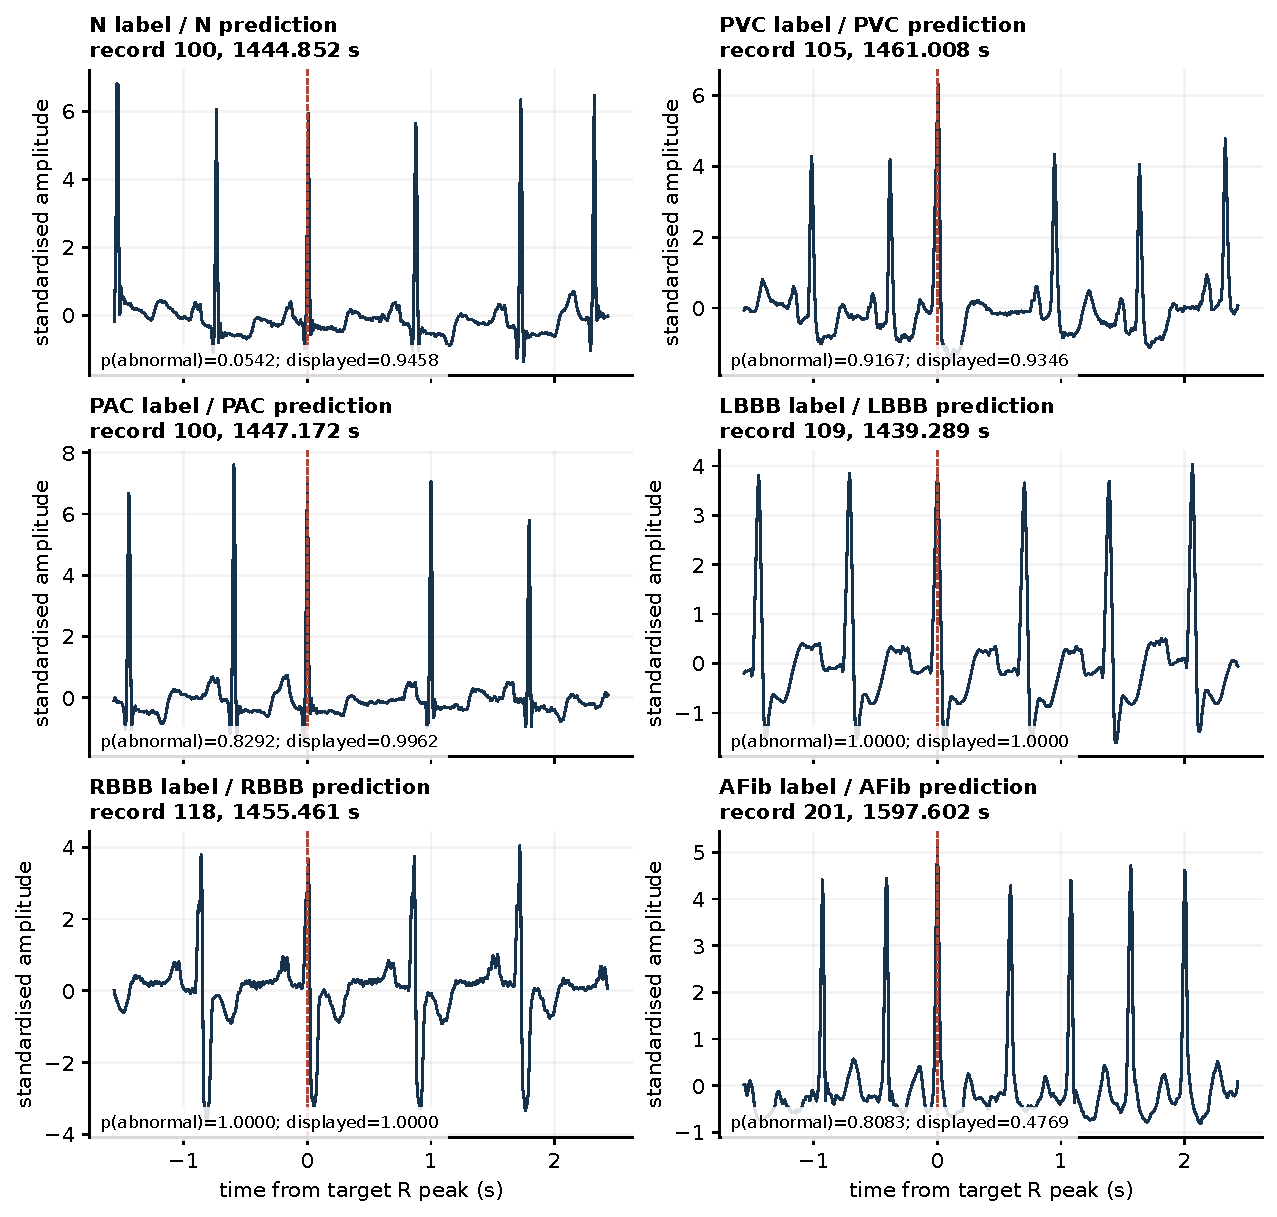
\includegraphics[width=.96\textwidth]{pic/generated/method_real_six_outputs.pdf}
\caption[Real temporal-test examples of all six outputs.]{Real prepared
four-second MLII windows illustrating the six project outputs. For each
class, the first correctly classified test example in saved order is shown;
the PVC additionally requires earlier fitting PVCs in the same record.
The dashed line marks the target beat. Scores are actual frozen-model
outputs. Selection for correct classification means this panel is an
explanation of behaviour, not evidence of perfect accuracy.}
\label{fig:method-real-six-outputs}
\end{figure}

\begin{table}[H]
\centering
\small
\caption{Measured predictions for the six real illustrative test segments.}
\label{tab:real-six-predictions}
\begin{tabular}{@{}llrrr@{}}
\toprule
Reference and output & Record & Peak time (s) & Binary score & Displayed score\\
\midrule
N & 100 & 1444.851563 & 0.054167 & 0.945833\\
PVC & 105 & 1461.007813 & 0.916667 & 0.934615\\
PAC & 100 & 1447.171875 & 0.829167 & 0.996154\\
LBBB & 109 & 1439.289063 & 1.000000 & 1.000000\\
RBBB & 118 & 1455.460938 & 1.000000 & 1.000000\\
AFib & 201 & 1597.601563 & 0.808333 & 0.476923\\
\bottomrule
\end{tabular}
\end{table}

The AFib example is especially informative: its subtype scores for AFib and
PAC are 0.476923 and 0.453846. AFib wins narrowly, even though its score is
below 0.5, because subtype selection uses the largest of five scores and
the final bundle disables low-confidence rejection. The reference AFib label
comes from the project's rhythm-annotation mapping, including its stated
AFIB/AFL grouping; a four-second plot alone is not used to establish that
label. Neither a score of 1 nor agreement in these selected examples is a
calibrated clinical certainty. The complete results, including errors, remain
in Chapter~\ref{ch:results}.

The complete operational sequence is therefore visible in measured data:
normal ECG supplies reconstruction targets; labelled earlier MLII beats
supply weighted binary and subtype fitting rows; validation chooses the
settings and gate; refitting produces fixed trees; and a later waveform
passes through preparation, feature construction, the gate, and subtype
selection. Prediction neither receives the expert label nor changes the
network weights or tree rules.

All numerical values, the full 242-entry rows, source locations, training
weights, and complete tree routes are retained in the audit file:
\par{\small\nolinkurl{experiments/methodology_real_case.json}}\par
The figures and numerical audit can be regenerated using:
\par{\small\nolinkurl{tools/generate_real_methodology_case.py}}\par
The audit records hashes
confirming that the original autoencoder and forest files were not modified.
